\documentclass[11pt,a4paper]{article}
\usepackage[utf8]{inputenc}
\usepackage[T1]{fontenc}
\usepackage{mathpazo}
\usepackage[a4paper,margin=2.5cm]{geometry}
\usepackage{amsmath,amssymb,amsthm,bm}
\usepackage{booktabs,tabularx}
\usepackage{graphicx}
\usepackage{float}
\usepackage[section]{placeins}
\usepackage[font=small,labelfont=bf]{caption}
\usepackage[round,authoryear]{natbib}
\usepackage[hidelinks]{hyperref}
\usepackage{enumitem}
\setlist{nosep,leftmargin=*}
\sloppy

\newtheorem{proposition}{Proposition}
\newcommand{\E}{\mathbb{E}}
\newcommand{\Var}{\operatorname{Var}}
\newcommand{\Cov}{\operatorname{Cov}}
\newcommand{\N}{\mathcal{N}}

\title{\textbf{Market Efficiency and a State-Space Model\\ of Team Strength}\\[6pt]
\large Evidence from Serie A odds and shots on target, 2020--2026}
\author{Alfredo Berlose}
\date{October 2026}

\begin{document}
\maketitle

\begin{abstract}
\noindent This paper studies whether a quantitative model built on public football data contains
information that betting odds do not already hold. The reference price is Pinnacle, whose closing
probabilities are shown to be well calibrated. Goal intensities are extracted from the odds in the
same way implied volatility is extracted from option prices, and the mispricing of the draw under
independent Poisson is corrected by the Dixon--Coles adjustment and by a bivariate Poisson model.
Team strength is then modelled as a latent state in a league-wide Kalman filter, estimated by maximum
likelihood on shots on target. All five parameters are estimated from the data, and the model passes
the standard diagnostics: the innovations are standard normal white noise, both in sample and out of
sample, with no volatility clustering. Two results follow. First, strength is almost constant within a
season, since the estimated drift is zero and values above $0.010$ are rejected. Second, over three
out-of-sample seasons the filter forecasts shots better than naive benchmarks, but it adds no
information to the odds, with a coefficient of $-0.027$ and a $p$-value of $0.73$ on 739 matches. A
walk-forward betting backtest confirms the result and shows that the only strategy with positive
closing line value would grow a bankroll by less than one percent per season. The model is therefore
useful as a measurement device rather than as a forecasting edge.
\end{abstract}

\tableofcontents
\newpage

%=====================================================================
\section{Introduction}
%=====================================================================
Betting markets are a natural laboratory for testing efficiency, because every contract has a known
expiry and a verifiable payoff. The question asked here is narrow and testable: does a model built on
publicly available football data contain information that the odds do not already incorporate? The
answer is negative, and this paper documents it with a protocol fixed in advance.

The study proceeds in three stages. The first stage treats the market as the underlying asset. Odds
are converted into probabilities, their calibration is checked, and goal intensities are extracted by
inversion. The second stage builds a state-space model of team strength and estimates it by maximum
likelihood. The third stage asks whether the model beats the market, both statistically and
economically, using only information available before kick-off.

Three features distinguish the empirical design. Every analysis follows a protocol written before the
results were seen, so thresholds and decision rules are not chosen after the fact. Every forecast uses
past matches only, with parameters re-estimated each summer under a frozen rule. Finally, the economic
evaluation reports closing line value rather than profit alone, because profit over a few hundred bets
is dominated by variance.

Our findings connect to a literature that generally supports the efficiency of major football betting
markets \citep{ers2020}, while the modelling framework follows the Poisson tradition of
\citet{maher1982} and \citet{dixoncoles1997}, and the state-space tradition of \citet{harvey1989} and
\citet{durbinkoopman2012}.

%=====================================================================
\section{Data and research design}
%=====================================================================
\subsection{Data}
Match data come from \texttt{football-data.co.uk}, with one file per Serie A season. Each record
contains goals, shots on target, and odds from several bookmakers, both at opening and at closing.
Three features of the data drive specific choices.

First, the season is taken from the first date of each file rather than from each match date, because
the 2019/20 season ran until August 2020. Second, the definition of shots on target changed after
2020/21, since the average fell from about $5.3$ to about $4.1$ per team; models based on shots
therefore use seasons from 2021/22 onwards. Third, Pinnacle odds are missing from January 2026, so
Betfair Exchange closing odds are used as a fallback.

\begin{table}[H]
\centering\small
\begin{tabular}{lrrrrr}
\toprule
Season & Matches & Goals per team & Shots on target & Home win rate & Pinnacle coverage \\
\midrule
2020/21 & 380 & 1.53 & 5.30 & 0.408 & 100\% \\
2021/22 & 380 & 1.43 & 4.44 & 0.389 & 100\% \\
2022/23 & 380 & 1.28 & 4.09 & 0.424 & 100\% \\
2023/24 & 380 & 1.31 & 4.15 & 0.418 & 100\% \\
2024/25 & 380 & 1.28 & 4.04 & 0.397 & 100\% \\
2025/26 & 380 & 1.21 & 4.03 & 0.389 & 52\% \\
2026/27 & 70 & 1.48 & 4.91 & 0.471 & 0\% \\
\bottomrule
\end{tabular}
\caption{Serie A data by season. The drop in shots on target after 2020/21 reflects a change in the
definition, not a change in play. The 2026/27 season is still in progress.}
\label{tab:data}
\end{table}

\subsection{Research design}
Seasons are divided in advance. The 2021/22 and 2022/23 seasons are used for estimation, 2023/24 for
validation, and 2024/25 together with 2025/26 for the final test, which was run once. The 2026/27
season is used only for the application in Section~\ref{sec:application}.

Model parameters are re-estimated every summer on the most recent season, under a rule chosen on the
validation sample and then frozen. Every forecast uses matches played strictly earlier, and state
estimates are taken as of the day the odds were collected.

%=====================================================================
\section{The market as a probability measure}
%=====================================================================
Decimal odds imply raw probabilities $1/o_k$ that sum to more than one, and the excess is the
bookmaker margin. The margin is removed proportionally, so that
\begin{equation}
\pi_k = \frac{1/o_k}{\sum_j 1/o_j}, \qquad m = \sum_j \frac{1}{o_j} - 1 .
\end{equation}
On Pinnacle closing odds from 2020/21 to 2024/25, covering 1{,}900 matches, the average margin is
$0.026$ with a range from $0.007$ to $0.059$. This margin is small by industry standards, which is
consistent with Pinnacle acting as a reference price.

Figure~\ref{fig:calibration} reports two checks. Panel (a) groups matches by predicted probability and
compares each group with the observed frequency; the points lie close to the diagonal across the whole
range. Panel (b) regresses the goal difference on the probability difference, giving a slope of $2.49$
and an $R^2$ of $0.26$. The low $R^2$ does not indicate a poorly priced market, because a single
football match is dominated by chance, and the remaining variance is largely irreducible.

\begin{figure}[H]
\centering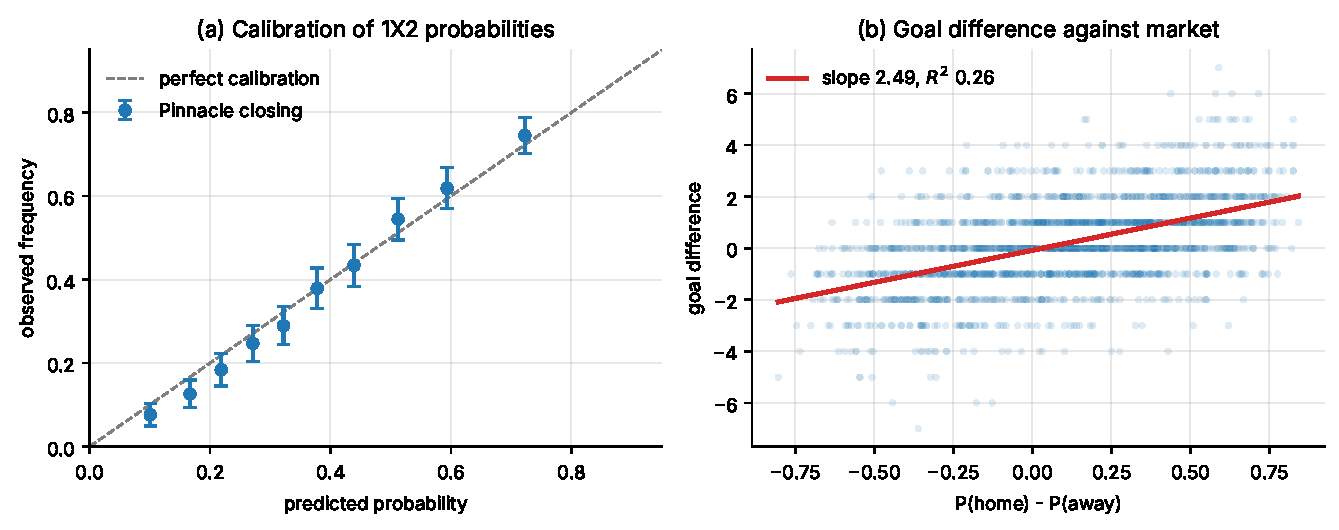
\includegraphics[width=\textwidth]{figures/fig1_calibration.pdf}
\caption{Calibration of Pinnacle closing odds, Serie A 2020/21--2024/25. Error bars show 95\%
confidence intervals for the observed frequency within each decile.}
\label{fig:calibration}
\end{figure}

\paragraph{Expected value.} For a bet at decimal odds $o$ with true probability $p$, the profit per
unit staked is $o-1$ with probability $p$ and $-1$ otherwise, so that
\begin{equation}
\E[\text{profit}] = p(o-1) + (1-p)(-1) = po - 1 .
\label{eq:ev}
\end{equation}
The fair price is therefore $1/p$, and a bet has positive expected value only when the offered odds
exceed it. This identity is used throughout Section~\ref{sec:betting}.

%=====================================================================
\section{Implied goal intensities}
%=====================================================================
\subsection{Inversion in two steps}
The approach mirrors implied volatility. A pricing model is inverted until it reproduces observed
prices, and the resulting parameters summarise what the market believes. Under independent Poisson
goals, the total follows a Poisson distribution with mean $T = \lambda_h + \lambda_a$, and the goal
difference follows a Skellam distribution. Two prices then identify two intensities:
\begin{enumerate}
\item the total $T$ solves $1 - F_{\text{Pois}}(2;T) = \pi_{\text{Over}}$, which has a unique root
because the left-hand side increases in $T$;
\item the split $s$, with $\lambda_h = sT$ and $\lambda_a = (1-s)T$, solves
$P(D>0) - P(D<0) = \pi_1 - \pi_2$, which increases in $s$.
\end{enumerate}
Both roots are found by Brent's method, and the procedure never fails on the 1{,}900 matches of the
estimation sample.

\subsection{The draw is mispriced, and by how much}
The draw is not used in the inversion, so its model price is an out-of-sample check. Under independent
Poisson the draw is underpriced by $2.26$ percentage points on average, as reported in
Table~\ref{tab:goals}. The deviation is systematic rather than random, which indicates that goals
scored by the two teams are not independent.

\subsection{Two corrections}
\citet{dixoncoles1997} multiply the probabilities of low scores by a factor $\tau$ that depends on a
single parameter $\rho$.

\begin{proposition}
The Dixon--Coles adjustment leaves $P(1)-P(2)$ and $P(\text{Over }2.5)$ unchanged, and modifies the
draw and the both-teams-to-score probability as follows:
\[
P_{DC}(X) = P_{\text{Pois}}(X) - 2\rho\,\lambda_h\lambda_a e^{-T}, \qquad
P_{DC}(BTTS) = P_{\text{Pois}}(BTTS) - \rho\,\lambda_h\lambda_a e^{-T}.
\]
\end{proposition}
\begin{proof}
The four adjusted cells have Poisson probabilities $e^{-T}$, $\lambda_a e^{-T}$, $\lambda_h e^{-T}$
and $\lambda_h\lambda_a e^{-T}$. The changes are $-\rho\lambda_h\lambda_a e^{-T}$ on $(0,0)$ and
$(1,1)$, and $+\rho\lambda_h\lambda_a e^{-T}$ on $(0,1)$ and $(1,0)$. A home win is affected only
through $(1,0)$ and an away win only through $(0,1)$, by the same amount, so their difference is
unchanged. All four cells contain at most two goals and the changes sum to zero, so the Over
probability is unchanged. The draw is affected through $(0,0)$ and $(1,1)$, and both teams scoring
only through $(1,1)$.
\end{proof}

The proposition yields a closed form for the implied $\rho$ of each match, namely
$\rho = (P_{\text{Pois}}(X) - \pi_X)/(2\lambda_h\lambda_a e^{-T})$. Its median is $-0.103$ and it is
stable across seasons, which suggests a structural feature rather than noise.

The bivariate Poisson model of \citet{karlis2003} writes goals as $X = X_1 + X_3$ and $Y = X_2 + X_3$,
where the three components are independent Poisson variables. The shared component $X_3$ adds one goal
to each side, so it raises the total without changing the difference, and the covariance equals $l_3$.
Three parameters then match three independent prices exactly. The median $l_3$ is $0.209$, implying a
correlation of about $0.16$, and the system has no solution in 30 matches out of 1{,}900.

\begin{table}[H]
\centering
\begin{tabular}{lrr}
\toprule
Model & Draw: model $-$ market (pp) & BTTS: model $-$ observed (pp) \\
\midrule
Independent Poisson & $-2.26$ & $-3.58$ \\
Dixon--Coles ($\rho = -0.103$) & $0.00$ & $-2.46$ \\
Bivariate Poisson & $0.00$ & $-0.60$ \\
\bottomrule
\end{tabular}
\caption{Model prices against the market, 1{,}900 matches. The draw is reproduced by construction once
a dependence parameter is added, but both-teams-to-score is not used in the calibration and therefore
remains an external check.}
\label{tab:goals}
\end{table}

\begin{figure}[H]
\centering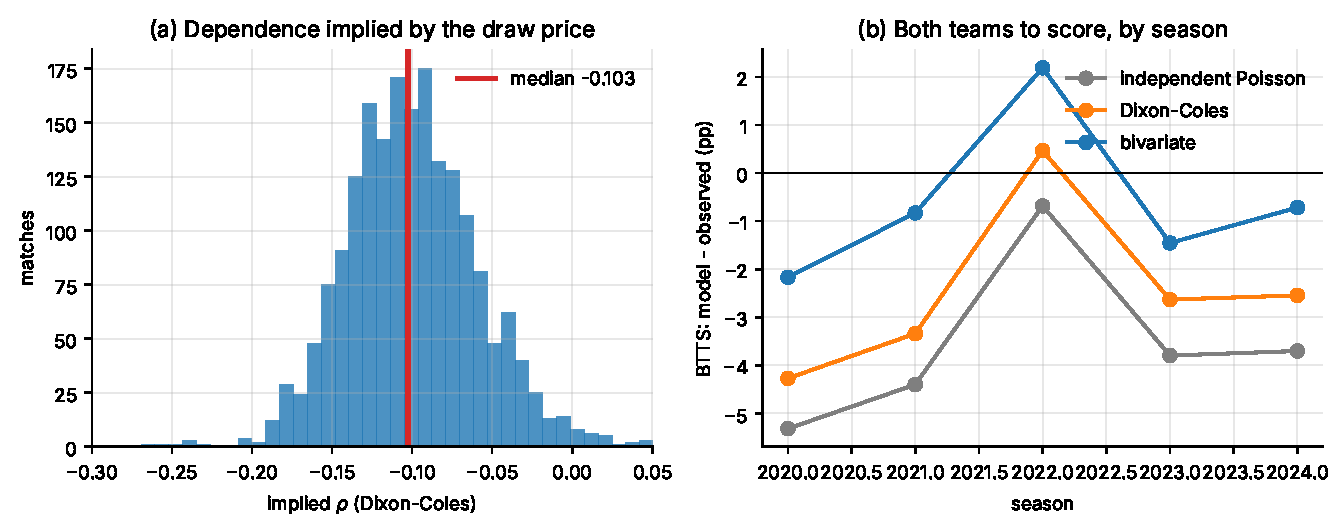
\includegraphics[width=\textwidth]{figures/fig2_goal_models.pdf}
\caption{Panel (a): distribution of the implied Dixon--Coles $\rho$ across matches. Panel (b): error on
both teams to score, by season and by model.}
\label{fig:goals}
\end{figure}

A caveat applies to the bivariate model. It was selected after the gap on both teams to score had been
observed, so its advantage on that market should be confirmed on new data before it is used.

%=====================================================================
\section{Is there momentum that the market misses?}
%=====================================================================
If teams went through periods of form that the market ignored, the gaps between outcomes and market
expectations would be autocorrelated. Five such gaps are constructed for each team and match: goals
scored and conceded relative to the implied intensities, shots on target relative to a season-specific
regression on those intensities, and goals relative to shots.

Autocorrelations are computed at lags one to five, with pairs taken only within the same team-season.
The null distribution comes from 1{,}000 permutations of the match order within each team-season, which
preserves the level of each team and destroys only the ordering in time. This design matters, because
short series produce a downward bias in the estimated autocorrelation, and the permutation
distribution reproduces that bias automatically.

\begin{table}[H]
\centering
\begin{tabular}{lrrr}
\toprule
Series & Mean ACF (lags 1--5) & Chance level & $p$-value \\
\midrule
Goals scored & $-0.0005$ & $-0.0011$ & 0.463 \\
Goals conceded & $-0.0065$ & $-0.0039$ & 0.633 \\
Shots on target, for & $0.0002$ & $0.0098$ & 0.890 \\
Shots on target, against & $0.0094$ & $0.0111$ & 0.581 \\
Conversion & $0.0221$ & $0.0138$ & 0.141 \\
\bottomrule
\end{tabular}
\caption{Persistence of gaps against the market, 3{,}040 team-matches in 80 team-seasons. With five
tests the Bonferroni threshold is $p < 0.010$. No series is persistent.}
\label{tab:persistence}
\end{table}

\begin{figure}[H]
\centering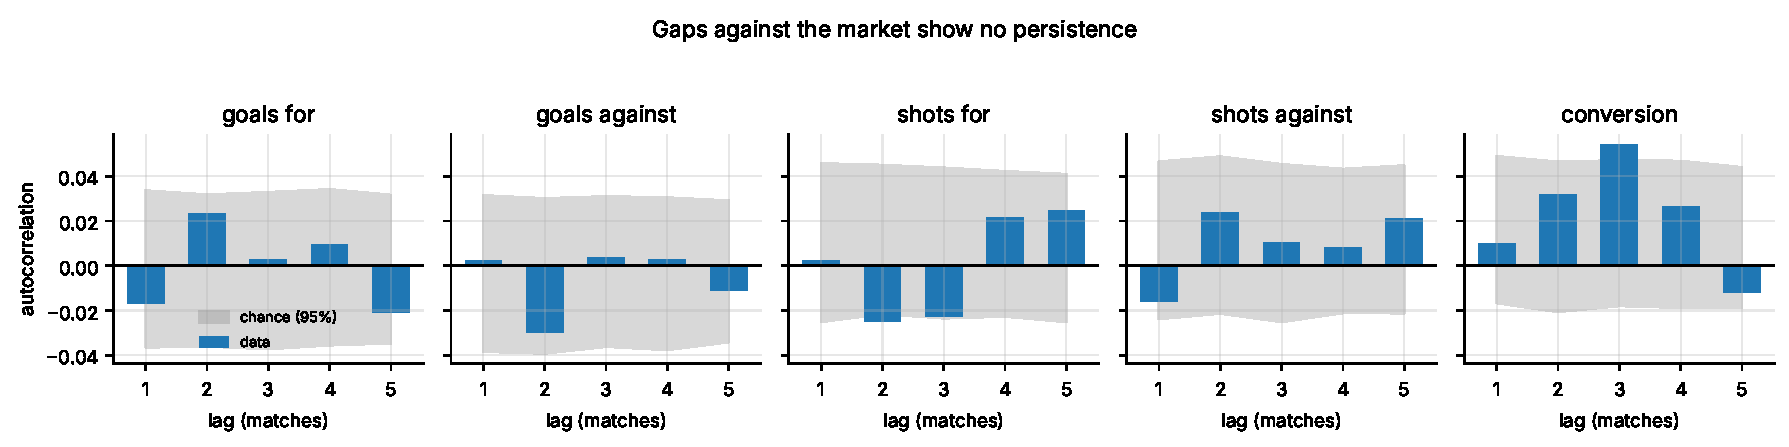
\includegraphics[width=\textwidth]{figures/fig3_persistence.pdf}
\caption{Autocorrelation of the gaps against the market, with the 95\% band from permutations. The band
lies slightly below zero because of the small-sample bias described in the text.}
\label{fig:persistence}
\end{figure}

The result is clear and it shapes the rest of the paper. Deviations from market expectations behave
like white noise, so a model of within-season form has little to capture. Attention therefore moves to
a model of the level of team strength.

%=====================================================================
\section{A state-space model of team strength}
%=====================================================================
\subsection{Specification}
Team strength is not observed, and single matches are noisy. This is the setting for which state-space
models were designed. The state is the vector $\bm\beta \in \mathbb{R}^{m}$ of strengths of all teams,
with a full covariance matrix $\bm P$. In match $t$ between team $i$ at home and team $j$ away,
\begin{equation}
y_t = \text{HST}_t - \text{AST}_t = \bm H_t \bm\beta + h + \varepsilon_t, \qquad
\bm H_t = \bm e_i^\top - \bm e_j^\top, \qquad \varepsilon_t \sim \N(0,R),
\end{equation}
where $h$ is the home advantage. Strength drifts by $\N(0,Q)$ each time a team plays, and by
$\N(0,Q_{\text{summer}})$ over the summer break. Promoted teams restart from the average of the
relegated teams with prior variance $P_0$.

The filter alternates prediction and updating:
\begin{align}
F_t &= P_{ii} + P_{jj} - 2P_{ij} + R, &
\bm K_t &= \frac{\bm P_{\cdot i} - \bm P_{\cdot j}}{F_t}, \\
v_t &= y_t - (b_i - b_j + h), &
\bm b &\leftarrow \bm b + \bm K_t v_t, \qquad \bm P \leftarrow \bm P - \bm K_t F_t \bm K_t^\top .
\end{align}
Here $v_t$ is the surprise, or innovation, and $F_t$ is the variance the filter announced for it. The
gain $\bm K_t$ has a direct interpretation, because it equals the ratio between what the filter does
not know and the total uncertainty of the forecast. It is therefore large at the start of a season and
small once evidence has accumulated.

Since the data only identify differences between teams, the common level is not identified. Strengths
are consequently reported as deviations from the league mean, with the corresponding transformation
applied to the covariance matrix.

\subsection{Estimation}
Estimation uses the prediction error decomposition. Under correct specification each innovation is
normal with the announced variance, so that
\begin{equation}
\log L = -\frac{1}{2}\sum_t \left[ \log(2\pi F_t) + \frac{v_t^2}{F_t} \right].
\label{eq:loglik}
\end{equation}
All five parameters are estimated by maximising \eqref{eq:loglik}, with variances parameterised in logs
so that they remain positive. No parameter is fixed by hand.

\begin{table}[H]
\centering
\begin{tabular}{lrl}
\toprule
Parameter & Estimate & Interpretation \\
\midrule
$Q$ & $0.0000$ & strength drift between two matches \\
$R$ & $9.63$ & noise of a single match ($\pm 3.10$ shots) \\
$h$ & $+0.525$ & home advantage in shots on target \\
$Q_{\text{summer}}$ & $0.042$ & strength drift over the summer \\
$P_0$ & $2.13$ & prior variance of strength ($\pm 1.46$ shots) \\
\bottomrule
\end{tabular}
\caption{Maximum likelihood estimates on 2021/22 and 2022/23, 760 matches.}
\label{tab:params}
\end{table}

The estimate of $P_0$ deserves a comment, because it is identified only by the first matchday and by
promoted teams. Its profile interval runs from $1.39$ to $3.63$, and the point estimate of $2.13$ is
close to the observed cross-sectional variance of strengths, which is $2.08$. The agreement is
reassuring, although the parameter remains the least precisely estimated of the five.

%=====================================================================
\section{Model comparison and diagnostics}
%=====================================================================
\subsection{Nested models}
Two restrictions are of interest. The first removes team strengths altogether, leaving home advantage
and noise. The second sets $Q = 0$, so that strength is constant within a season.

\begin{table}[H]
\centering
\begin{tabular}{lrrrr}
\toprule
Model & $\log L$ & Parameters & AIC & BIC \\
\midrule
No team strength ($h$ + noise) & $-2085.90$ & 2 & 4175.81 & 4185.07 \\
Constant strength ($Q = 0$) & $-1970.19$ & 4 & \textbf{3948.38} & \textbf{3966.91} \\
Full model ($Q$ free) & $-1970.19$ & 5 & 3950.38 & 3973.54 \\
\bottomrule
\end{tabular}
\caption{Model comparison on 760 matches. Lower values of AIC and BIC are preferred.}
\label{tab:aic}
\end{table}

Team strengths are strongly supported, since the likelihood ratio statistic is $231.4$ on one degree
of freedom, with a $p$-value of about $3 \times 10^{-52}$. The drift parameter is not supported. Its
likelihood ratio statistic is zero, and because $Q = 0$ lies on the boundary of the parameter space the
null distribution is the mixture $\tfrac12\chi^2_0 + \tfrac12\chi^2_1$ of \citet{selfliang1987}, which
gives $p = 0.50$. Both AIC and BIC prefer the restricted model.

The profile likelihood in Figure~\ref{fig:profiles} gives the same message in a different form. Values
of $Q$ up to $0.010$ are compatible with the data at the 95\% level, which corresponds to at most
$\pm 0.62$ shots of drift over an entire season. Strength behaves as a trait rather than as a form
cycle, and this is consistent with the permutation tests of the previous section.

\begin{figure}[H]
\centering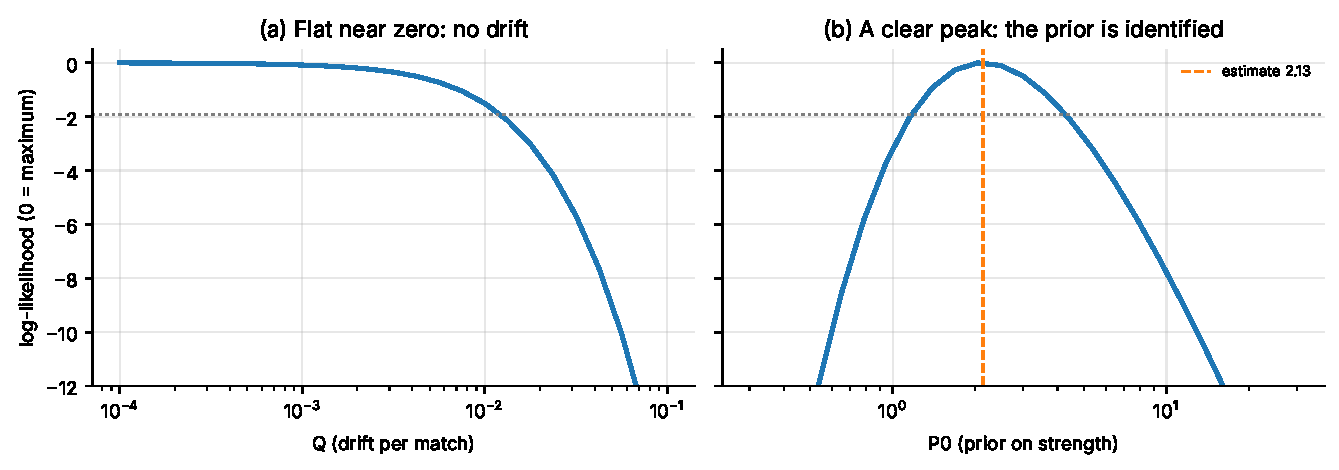
\includegraphics[width=0.9\textwidth]{figures/fig4d_profiles.pdf}
\caption{Profile log-likelihoods. The horizontal line is the 95\% threshold of $-1.92$, that is half
the $\chi^2_1$ quantile. Panel (a) is flat near zero, so the drift is not identified away from zero.
Panel (b) has a clear interior peak.}
\label{fig:profiles}
\end{figure}

\subsection{Variance decomposition}
The model implies a decomposition of the variance of the shot difference into a part explained by
strengths and home advantage, and an irreducible part:
\begin{equation}
\Var(y) = \Var(\beta_i - \beta_j + h) + R, \qquad 14.17 = 3.78 \;(27\%) + 9.63 \;(73\%).
\end{equation}
The filter therefore absorbs about one quarter of the variability, and the rest is the randomness of a
single match. This is not a shortcoming, because the model is not required to remove that randomness.
It is required to measure it correctly, which the diagnostics below confirm.

A second decomposition describes learning. The announced forecast variance splits into uncertainty
about strengths and match noise. Over the first 38 matches it averages $13.08 = 3.44 + 9.63$, and over
the last 38 matches it averages $9.93 = 0.29 + 9.63$. Almost all the initial ignorance has been
removed, and what remains is chance.

\begin{figure}[H]
\centering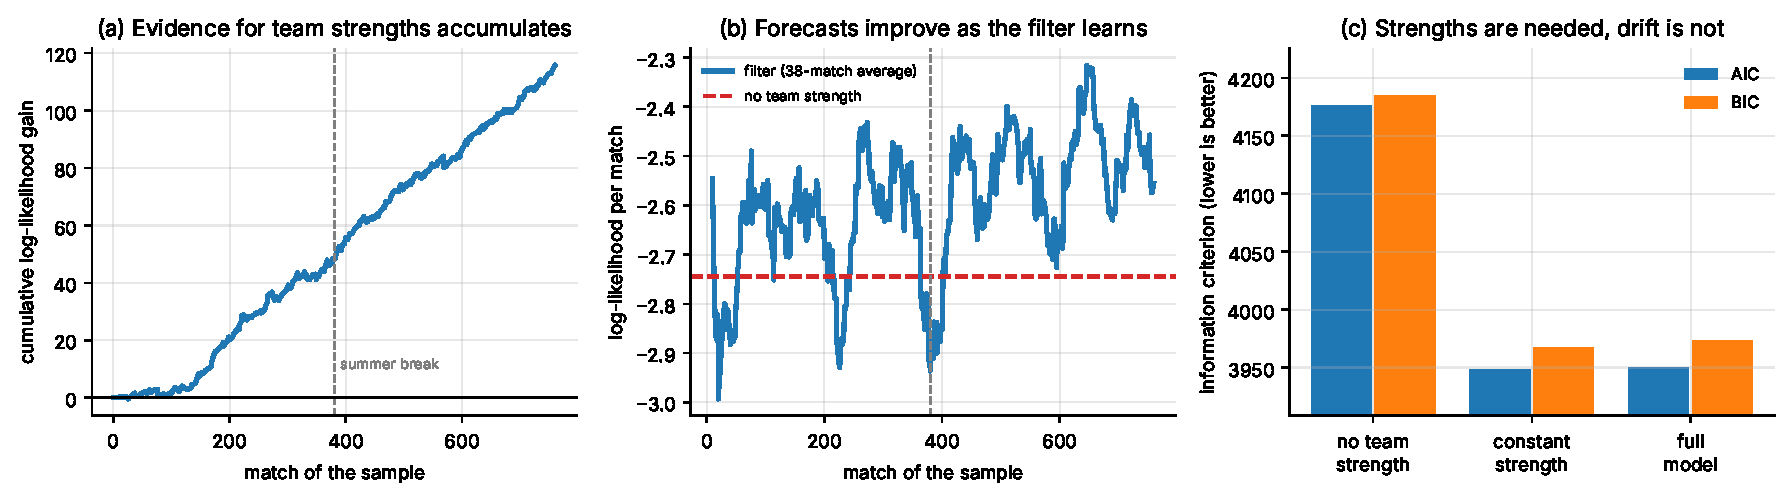
\includegraphics[width=\textwidth]{figures/fig4c_evidence.pdf}
\caption{Panel (a): log-likelihood accumulated against the model without team strengths. Panel (b):
log-likelihood per match, as a 38-match moving average, against the same benchmark. Panel (c):
information criteria for the three nested models.}
\label{fig:evidence}
\end{figure}

\subsection{Innovations}
A state-space model is judged by its innovations. If the specification is correct, the standardised
innovations $z_t = v_t / \sqrt{F_t}$ are standard normal and serially independent. The same logic
applies to a GARCH model, where standardised residuals are inspected after estimation.

\begin{table}[H]
\centering\small
\begin{tabular}{lrrrrrrrr}
\toprule
Sample & $n$ & Mean & Variance & Skewness & Exc. kurtosis & Jarque--Bera $p$ & Ljung--Box $p$ & ARCH-LM $p$ \\
\midrule
In sample & 760 & $0.002$ & $1.000$ & $-0.007$ & $0.330$ & 0.177 & 0.799 & 0.311 \\
Out of sample & 760 & $-0.032$ & $1.129$ & $-0.061$ & $-0.072$ & 0.727 & 0.127 & 0.680 \\
\bottomrule
\end{tabular}
\caption{Diagnostics on the standardised innovations. Ljung--Box and ARCH-LM use five lags. The
out-of-sample column refers to the 2024/25 and 2025/26 seasons.}
\label{tab:innovations}
\end{table}

All four requirements are met, and they are met out of sample as well. The mean and variance confirm
that the announced bands are honest. Normality supports the Gaussian likelihood, which matters because
the bands are the main output of the filter. Independence confirms that no predictable structure has
been left in the residuals. The ARCH test is also passed, so there is no volatility clustering and a
constant $R$ is adequate. Unlike financial returns, match noise in football appears homoskedastic, and
a GARCH component is therefore unnecessary.

\begin{figure}[H]
\centering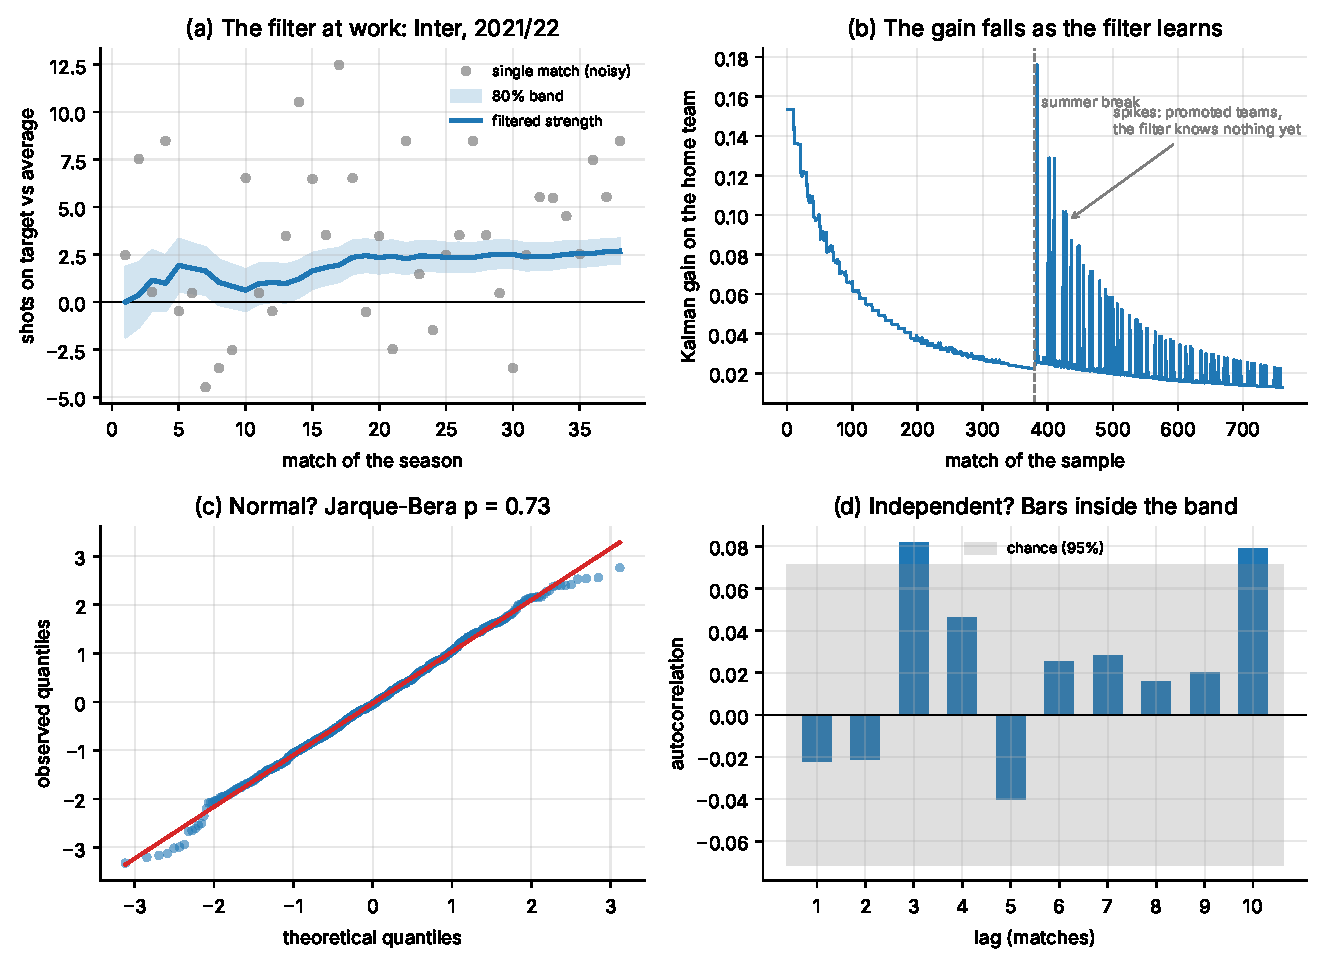
\includegraphics[width=\textwidth]{figures/fig4b_diagnostics.pdf}
\caption{Panel (a): filtered strength of one team against the matches it is estimated from. Panel (b):
the Kalman gain over the estimation sample; the spikes after the summer break are promoted teams.
Panels (c) and (d): normality and independence of the out-of-sample innovations.}
\label{fig:diagnostics}
\end{figure}

\begin{figure}[H]
\centering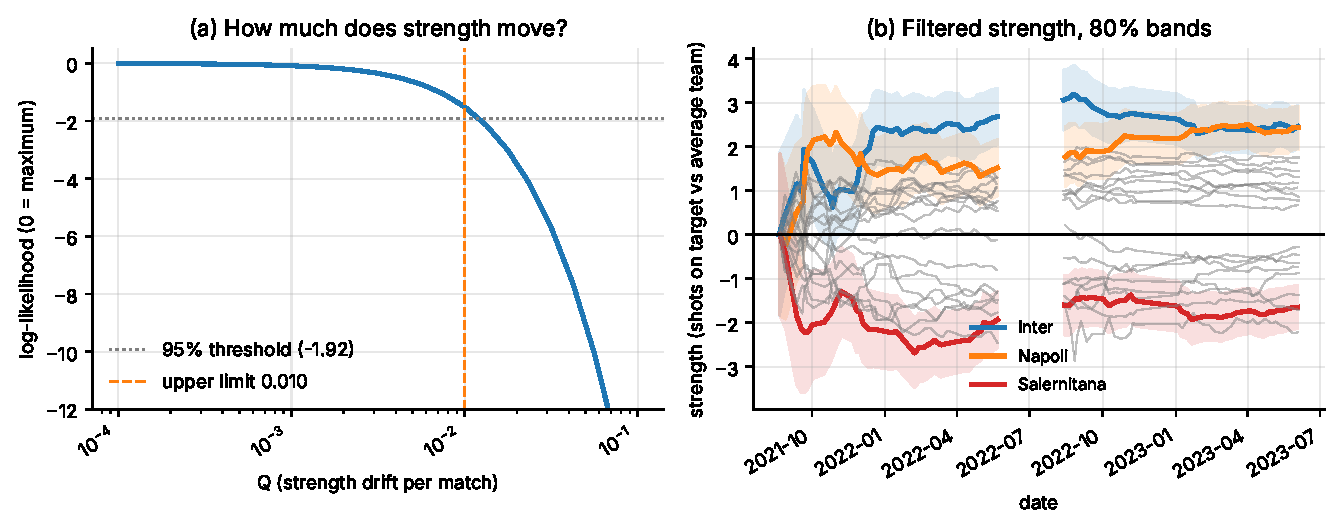
\includegraphics[width=\textwidth]{figures/fig4_kalman.pdf}
\caption{Panel (a): profile likelihood for the drift parameter. Panel (b): filtered strengths of all
teams, with 80\% bands for three of them.}
\label{fig:kalman}
\end{figure}

%=====================================================================
\section{Out-of-sample validation and test}
%=====================================================================
Parameters are re-estimated each summer on the most recent season, under a rule selected on the
validation season and then frozen. Every forecast uses only matches played earlier. Three questions are
asked in sequence.

\begin{table}[H]
\centering\small
\begin{tabular}{lrrrrrrr}
\toprule
& \multicolumn{2}{c}{Parameters} & \multicolumn{2}{c}{Uncertainty} & \multicolumn{3}{c}{RMSE} \\
\cmidrule(lr){2-3}\cmidrule(lr){4-5}\cmidrule(lr){6-8}
Season & $R$ & $h$ & Var($z$) & 80\% cover & Kalman & Season mean & Elo on shots \\
\midrule
2023/24 (validation) & 8.44 & $+0.55$ & 0.90 & 81.6\% & 2.854 & 3.094$^{*}$ & 2.856 \\
2024/25 (test) & 7.22 & $+0.96$ & 1.10 & 77.6\% & 2.984 & 3.179$^{*}$ & 2.986 \\
2025/26 (test) & 8.11 & $+0.51$ & 1.12 & 73.4\% & 3.120 & 3.360$^{*}$ & 3.134 \\
\bottomrule
\end{tabular}
\caption{Out-of-sample forecasting of the shot difference. An asterisk marks a difference from the
Kalman filter that is significant at the 5\% level, using weekly averages of the loss differential in
the spirit of \citet{dieboldmariano1995}. A model using home advantage only is also rejected in every
season, with $p < 0.001$.}
\label{tab:oos}
\end{table}

The uncertainty bands are close to their nominal level, and they are slightly narrow in the test
seasons. The main reason is that $R$ and $h$ vary across seasons, and a one-season window follows that
variation with a delay.

On accuracy, the filter clearly beats the naive benchmarks. It does not beat a well-tuned Elo rule on
the same data, which is expected: with $Q$ close to zero the Kalman gain converges to a constant, and a
fixed-gain rule becomes nearly equivalent. What the filter adds is not point accuracy but a stated and
verified uncertainty.

\paragraph{Does the filter add information to the odds?} The question is answered with an encompassing
regression of the goal difference on the market forecast and on the filter forecast, with one constant
per season and heteroskedasticity-robust standard errors \citep{white1980}:
\begin{equation}
\text{GF}_t - \text{GA}_t = a_s + b\,(\lambda_{h,t} - \lambda_{a,t}) + c\,\hat y^{K}_t + u_t .
\end{equation}
On 739 test matches the market coefficient is $1.084$ with $p < 0.001$, while the filter coefficient is
$-0.027$ with $p = 0.73$. The correlation between the two forecasts is $0.93$. The filter therefore
adds nothing once the odds are known, and the two forecasts say almost the same thing.

\begin{figure}[H]
\centering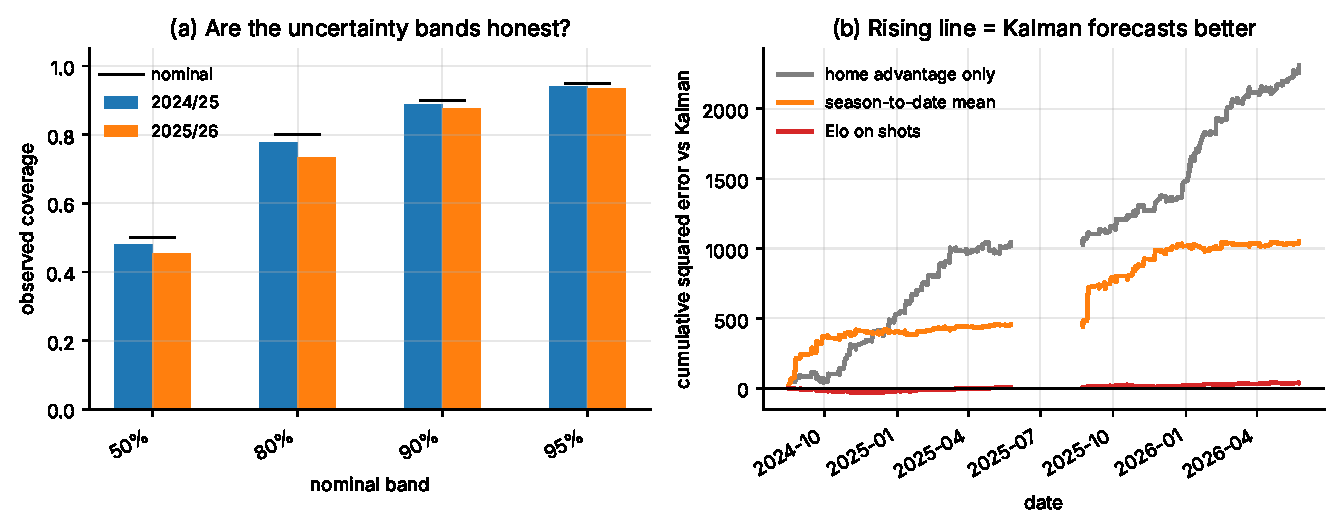
\includegraphics[width=\textwidth]{figures/fig5_outofsample.pdf}
\caption{Panel (a): nominal against observed coverage of the uncertainty bands. Panel (b): cumulative
squared error of each benchmark relative to the filter, so a rising line favours the filter.}
\label{fig:oos}
\end{figure}

%=====================================================================
\section{Economic evaluation}
\label{sec:betting}
%=====================================================================
\subsection{Design}
The backtest uses only information available on Friday. The reference price is Pinnacle before closing,
with Betfair Exchange as a fallback, and bets are placed at Bet365 Friday odds. Closing odds are used
exclusively to compute closing line value, defined as $o \cdot \pi^{\text{close}} - 1$, which measures
the quality of the price obtained rather than the outcome of the bet.

Three strategies are compared. The first uses market probabilities only. The second allows the filter
to shift those probabilities, through one weight per outcome estimated on earlier seasons with the
market probabilities entering as an offset. The third always backs the favourite and serves as a
control. The estimated weights are negative, at $-0.038$ and $-0.135$, which already indicates that the
filter carries no usable signal.

Two measures do not depend on the stake and therefore carry the test, namely the yield per euro staked
and the closing line value.

\begin{table}[H]
\centering\small
\begin{tabular}{lrrrrrrrr}
\toprule
Strategy & Bets & Draw share & Mean odds & Mean EV & Yield & $p$ & CLV & $p$ \\
\midrule
Market only & 74 & 31\% & 7.15 & $0.034$ & $-13.8\%$ & 0.73 & $\mathbf{+1.2\%}$ & 0.20 \\
Market + filter & 454 & 64\% & 3.20 & $0.036$ & $+11.4\%$ & 0.06 & $-2.3\%$ & 1.00 \\
Favourite (control) & 739 & 0\% & 1.91 & $-0.049$ & $-2.8\%$ & 0.79 & $-5.3\%$ & 1.00 \\
\bottomrule
\end{tabular}
\caption{Betting results over 71 matchdays and 739 matches. One-sided $p$-values; with three strategies
the corrected threshold is $0.017$. No strategy passes it.}
\label{tab:betting}
\end{table}

\subsection{A positive yield is not an edge}
The second strategy shows a yield of $+11.4\%$, which looks attractive at first sight. Three pieces of
evidence show that it is an artefact. First, the estimated filter weights are negative, so the strategy
effectively bets against the filter and inflates the draw probability. Second, it places 64\% of its
bets on the draw, which reflects a training sample in which draws were slightly more frequent than the
market implied. Third, and decisively, its closing line value is $-2.3\%$ with a $t$-statistic of
$-7.8$, which means the prices obtained were systematically worse than the closing price. A genuine
edge does not coexist with a strongly negative closing line value.

A paired test on the 46 matchdays where both strategies bet gives a difference of $+0.269$ per euro
staked with a $p$-value of $0.183$, so the apparent advantage is not significant. The test is
constructed on returns per euro staked, which makes it invariant to the staking rule.

\subsection{Is the surviving edge usable?}
Only the first strategy has positive closing line value, and its size can be assessed with the Kelly
growth rate, which does not depend on the size of the bankroll. For a bet at odds $o$ with edge
$\text{EV}$, the optimal fraction is $f^\star = \text{EV}/(o-1)$, and the expected growth of the log
bankroll follows from it. The estimated edge is shrunk by $0.51$, which is the ratio of closing line
value to expected value measured on the training seasons.

\begin{table}[H]
\centering
\begin{tabular}{llrr}
\toprule
Edge used & Kelly fraction & Growth per season & Median stake (\% of bankroll) \\
\midrule
As estimated & Full & $+0.55\%$ & 0.383 \\
As estimated & Quarter & $+0.24\%$ & 0.096 \\
Shrunk ($0.51$) & Full & $+0.14\%$ & 0.196 \\
Shrunk ($0.51$) & Quarter & $+0.06\%$ & 0.049 \\
\bottomrule
\end{tabular}
\caption{Growth of the market-only strategy, which is the one with positive closing line value. The
figures are independent of the size of the bankroll.}
\label{tab:kelly}
\end{table}

Even under full Kelly and with the edge taken at face value, growth is below one percent per season.
The reason lies in the formula: the strategy produces about 37 bets per season at average odds of
$7.15$, so the edge enters squared while the variance enters in the denominator.

A practical constraint reinforces the conclusion. Under quarter Kelly on the shrunk edge, the median
stake is $0.049\%$ of the bankroll, so a bankroll of about $4{,}100$ euro is needed before the median
stake reaches a typical minimum bet of two euro. With smaller bankrolls the strategy cannot be
implemented as specified, and betting the minimum instead would mean staking many times the Kelly
fraction.

\begin{figure}[H]
\centering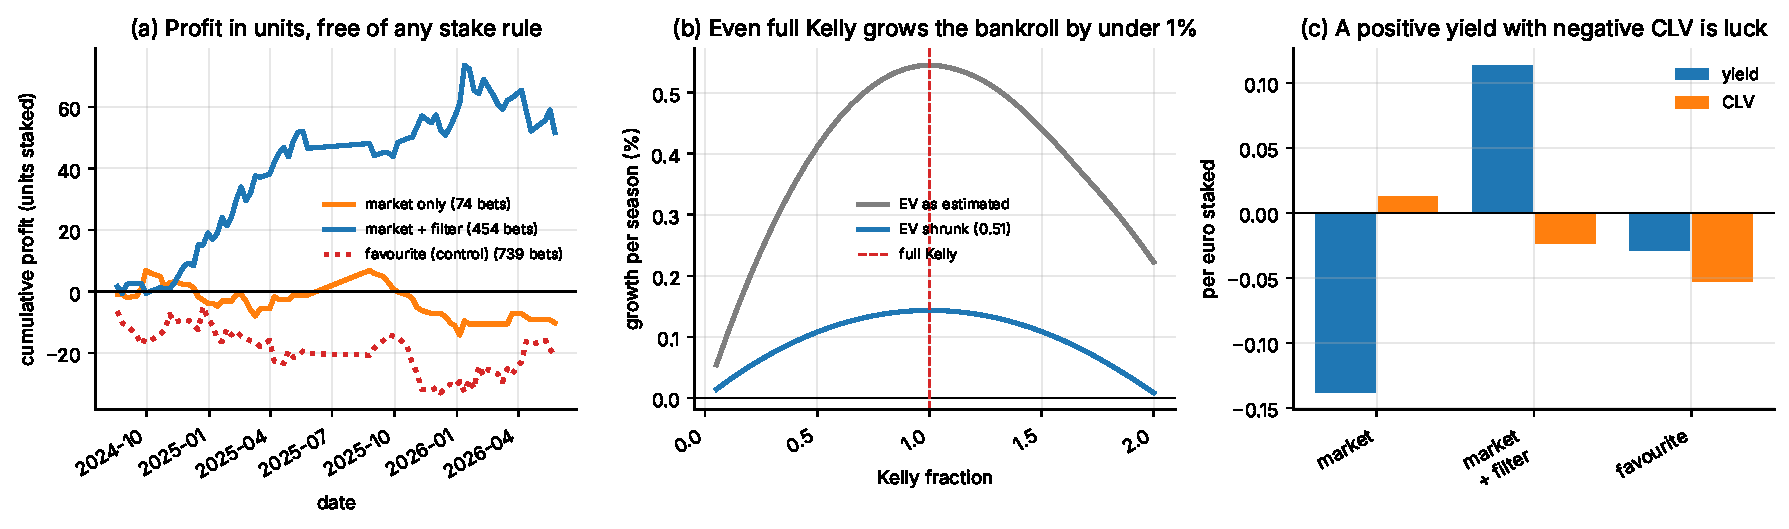
\includegraphics[width=\textwidth]{figures/fig6_betting.pdf}
\caption{Panel (a): cumulative profit in units staked, which is free of any staking rule. Panel (b):
growth per season as a function of the Kelly fraction. Panel (c): yield against closing line value.}
\label{fig:betting}
\end{figure}

%=====================================================================
\section{Application: reading a season in progress}
\label{sec:application}
%=====================================================================
The filter does not beat the market, but it measures team strength with a stated error, and that is
sufficient for a descriptive use. Two quantities are computed for the current season, after rescaling
shots on target because their level changed again in 2026/27.

Expected points come from the market. For the home team each match pays $3$, $1$ or $0$ with
probabilities $\pi_1$, $\pi_X$ and $\pi_2$, so that
\begin{equation}
z_{\text{points}} = \frac{\sum_t \left(\text{pt}_t - \E[\text{pt}_t]\right)}
{\sqrt{\sum_t \left(\E[\text{pt}_t^2] - \E[\text{pt}_t]^2\right)}} .
\end{equation}
Conversion luck treats each shot on target as a Bernoulli trial with success probability $c$, the
league conversion rate, which gives
\begin{equation}
z_{\text{conv}} = \frac{(G_F - cS_F) - (G_A - cS_A)}{\sqrt{c(1-c)(S_F + S_A)}} .
\end{equation}
Because conversion does not persist, as shown in Table~\ref{tab:persistence}, a large value of
$z_{\text{conv}}$ indicates luck that is unlikely to continue. With twenty teams the corrected
threshold is $3.02$.

\begin{table}[H]
\centering\small
\begin{tabular}{lrrrrrr}
\toprule
Team & Points & Expected & $z$ points & Rank by points & Rank by filter & $z$ conversion \\
\midrule
Inter & 19 & 15.5 & $+1.21$ & 1 & 1 & $+1.04$ \\
Juventus & 11 & 14.5 & $-1.10$ & 8 & 2 & $-1.58$ \\
Como & 14 & 12.8 & $+0.37$ & 5 & 3 & $-0.41$ \\
Roma & 17 & 12.8 & $+1.29$ & 3 & 4 & $+1.90$ \\
\textbf{Lazio} & \textbf{19} & \textbf{9.6} & $\mathbf{+2.89}$ & \textbf{1} & \textbf{8} & $\mathbf{+3.10}$ \\
Fiorentina & 4 & 9.7 & $-1.73$ & 16 & 10 & $-2.25$ \\
Venezia & 3 & 7.6 & $-1.46$ & 20 & 20 & $-0.89$ \\
\bottomrule
\end{tabular}
\caption{Selected teams from the 2026/27 season after 70 matches. Lazio is the only team whose
conversion exceeds the threshold corrected for twenty comparisons.}
\label{tab:application}
\end{table}

The table separates production from results. Lazio leads on points but ranks eighth on shots, and its
conversion is the only value above the corrected threshold, so part of its position is likely to be
temporary. Juventus shows the opposite pattern, since it ranks second on shots and eighth on points.

\begin{figure}[H]
\centering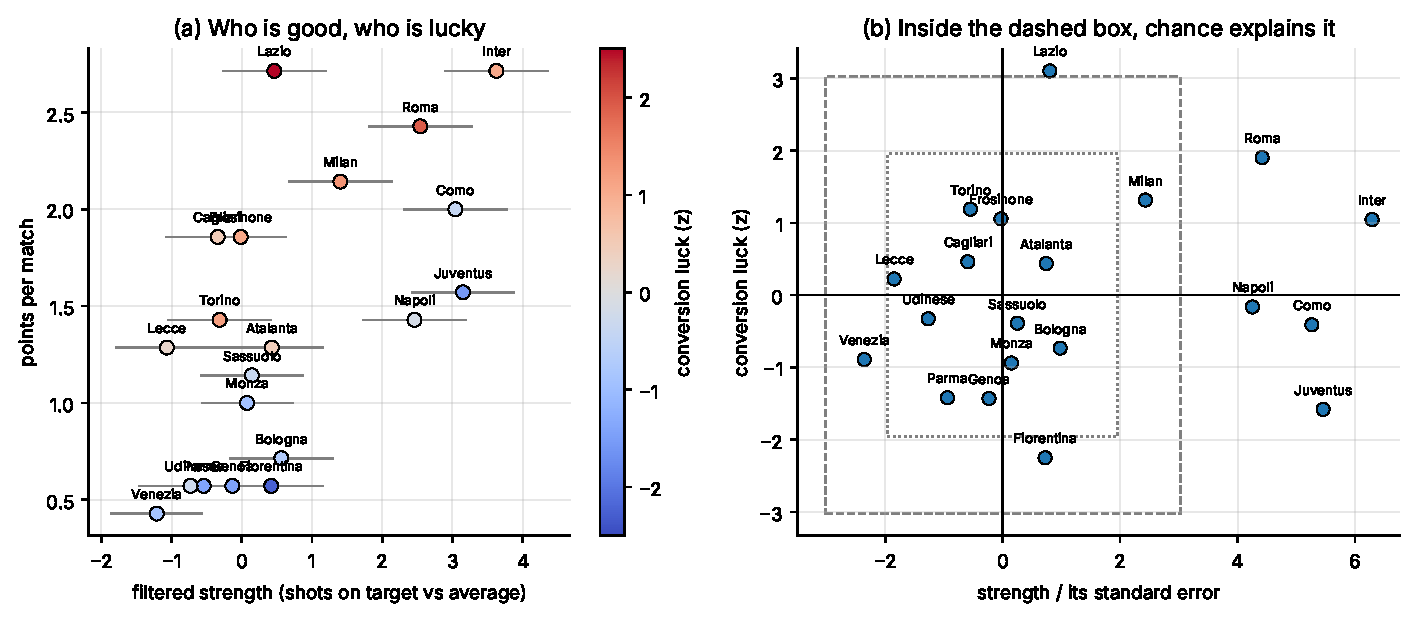
\includegraphics[width=\textwidth]{figures/fig7_application.pdf}
\caption{Panel (a): points per match against filtered strength, with colour showing conversion luck.
Panel (b): standardised strength against conversion luck, with the simple and the corrected thresholds.}
\label{fig:application}
\end{figure}

An event study supports this reading. Teams in the same position as Lazio, that is with conversion above
two standard errors and production below expectation, were identified in earlier seasons. Over the
following five matches their points fell from $2.18$ to $1.58$ per match, and their conversion returned
to normal. The market, however, had already priced the change, since those teams earned almost exactly
the points the odds implied, with a difference of $+0.03$ and a $t$-statistic of $0.25$.

%=====================================================================
\section{Conclusion}
%=====================================================================
Five results emerge from the study.

\begin{enumerate}
\item Pinnacle closing probabilities are well calibrated, and the margin is small and stable.
\item Goal intensities can be extracted from the odds exactly. The mispricing of the draw under
independent Poisson reveals dependence between the goals of the two teams, which Dixon--Coles captures
with a stable $\rho \approx -0.10$ and the bivariate model with $l_3 \approx 0.21$.
\item Deviations from market expectations show no persistence, in the mean or in the variance.
\item Team strength measured by shots on target is almost constant within a season, since the drift is
estimated at zero and values above $0.010$ are rejected.
\item Over three out-of-sample seasons the filter forecasts shots better than naive benchmarks, but it
adds no information to the odds, and the only strategy with positive closing line value would grow a
bankroll by less than one percent per season.
\end{enumerate}

The contribution is therefore twofold. On the substantive side, the paper provides evidence that the
Serie A betting market is efficient with respect to public match data, even on Friday prices rather
than closing prices. On the methodological side, it shows that a state-space model remains valuable
when it does not beat the market, because it measures strength with a verified uncertainty and
separates production from luck.

Several extensions would strengthen the analysis. Separate attack and defence states would describe
the shape of a match rather than only its balance. Additional leagues would provide more validation
seasons, and would allow the bivariate model to be confirmed on both teams to score. Finally, a forward
register of recommendations would replace backtesting with a genuine out-of-sample record.

\begin{thebibliography}{99}
\bibitem[Diebold and Mariano(1995)]{dieboldmariano1995} Diebold, F.~X. and Mariano, R.~S. (1995).
Comparing predictive accuracy. \emph{Journal of Business \& Economic Statistics}, 13(3), 253--263.
\bibitem[Dixon and Coles(1997)]{dixoncoles1997} Dixon, M.~J. and Coles, S.~G. (1997). Modelling
association football scores and inefficiencies in the football betting market. \emph{Journal of the
Royal Statistical Society, Series C}, 46(2), 265--280.
\bibitem[Durbin and Koopman(2012)]{durbinkoopman2012} Durbin, J. and Koopman, S.~J. (2012).
\emph{Time Series Analysis by State Space Methods}, 2nd edition. Oxford University Press.
\bibitem[Elaad et al.(2020)]{ers2020} Elaad, G., Reade, J.~J. and Singleton, C. (2020). Information,
prices and efficiency in an online betting market. \emph{Finance Research Letters}, 35, 101291.
\bibitem[Harvey(1989)]{harvey1989} Harvey, A.~C. (1989). \emph{Forecasting, Structural Time Series
Models and the Kalman Filter}. Cambridge University Press.
\bibitem[Hvattum and Arntzen(2010)]{hvattum2010} Hvattum, L.~M. and Arntzen, H. (2010). Using ELO
ratings for match result prediction in association football. \emph{International Journal of
Forecasting}, 26(3), 460--470.
\bibitem[Kalman(1960)]{kalman1960} Kalman, R.~E. (1960). A new approach to linear filtering and
prediction problems. \emph{Journal of Basic Engineering}, 82(1), 35--45.
\bibitem[Karlis and Ntzoufras(2003)]{karlis2003} Karlis, D. and Ntzoufras, I. (2003). Analysis of
sports data by using bivariate Poisson models. \emph{Journal of the Royal Statistical Society, Series
D}, 52(3), 381--393.
\bibitem[Maher(1982)]{maher1982} Maher, M.~J. (1982). Modelling association football scores.
\emph{Statistica Neerlandica}, 36(3), 109--118.
\bibitem[Self and Liang(1987)]{selfliang1987} Self, S.~G. and Liang, K.-Y. (1987). Asymptotic
properties of maximum likelihood estimators and likelihood ratio tests under nonstandard conditions.
\emph{Journal of the American Statistical Association}, 82(398), 605--610.
\bibitem[White(1980)]{white1980} White, H. (1980). A heteroskedasticity-consistent covariance matrix
estimator and a direct test for heteroskedasticity. \emph{Econometrica}, 48(4), 817--838.
\end{thebibliography}

\end{document}
